%%「論文」,「レター」,「レター(C分冊)」,「技術研究報告」などのテンプレート
%% v3.3 [2020/06/02]

\documentclass[technicalreport]{ieicej}
\usepackage[dvipdfmx]{graphicx,xcolor}
\usepackage{float}
\usepackage[fleqn]{amsmath}
\usepackage{newtxtext}% 英数字フォントの設定を変更しないでください
\usepackage[varg]{newtxmath}% % 英数字フォントの設定を変更しないでください
\usepackage{latexsym}
\usepackage{listings}
\usepackage{xurl}
\usepackage{fancyvrb}
\usepackage{multirow}
\usepackage{array}
\usepackage[section]{placeins} % make sure all fig and table do not go to other sections
\usepackage{stfloats} % somehow avoid the possible blank page by fig or table
% \usepackage[normalem]{ulem}
% \useunder{\uline}{\ul}{}
%\usepackage{amssymb}


\renewcommand{\refname}{References} % To get english reference section heading
\renewcommand{\figurename}{Fig.} % To get english figure heading
\renewcommand{\tablename}{Table} % To get english table heading
\renewcommand\UrlFont{\rmfamily} % Fix url font

\lstset{%
    language={Python},
    basicstyle={\small},%
    identifierstyle={\small},%
    commentstyle={\small\itshape},%
    keywordstyle={\small\bfseries},%
    ndkeywordstyle={\small},%
    stringstyle={\small\ttfamily},
    frame={tb},
    breaklines=true,
    columns=[l]{fullflexible},%
    numbers=left,%
    xrightmargin=0zw,%
    xleftmargin=3zw,%
    numberstyle={\scriptsize},%
    stepnumber=1,
    showstringspaces=false,%
    numbersep=1zw,%
    lineskip=-0.5ex,%
    %moredelim=[is][\underbar]{_}{_},%
    keepspaces=true,%
    %escapechar=\@
}

% \jtitle{タイトル}
% \jsubtitle{}
\etitle{A Study of Product Identification System Using Optical Character Recognition}
% \esubtitle{}
\authorlist{%
 \authorentry[chin-shiji@s.okayama-u.ac.jp]{陳 仕璽}{Shixi Chen}{okayama}
 \authorentry[funabiki@okayama-u.ac.jp]{舩曵 信生}{Nobuo Funabiki}{okayama}
 \authorentry[phvf8tn3@s.okayama-u.ac.jp]{坂上 正規}{Masaki Sakagami}{okayama}
 \authorentry[toshida.takashi@astrolab.co.jp]{土信田 高}{Takashi Toshida}{astrolab}
 \authorentry[suga@astrolab.co.jp]{菅 恒平}{Kohei Suga}{astrolab}
% \authorentry[メールアドレス]{和文著者名}{英文著者名}{所属ラベル}
}
\affiliate[okayama]{}
{Okayama University\hskip1em
Tsushimanaka 3-1-1, Okayama, 700--8530, Japan}
\affiliate[astrolab]{}
{Astrolab \hskip1em
Otemachi 2-6-2, Chiyoda, Tokyo, 100-0004, Japan}
%\affiliate[所属ラベル]{和文勤務先\\ 連絡先住所}{英文勤務先\\ 英文連絡先住所}
\jalcdoi{???????????}% ← このままにしておいてください

\begin{document}
% \begin{jabstract}
% %和文あらまし
% \end{jabstract}
% \begin{jkeyword}
% %和文キーワード
% \end{jkeyword}

\begin{eabstract}
    %background
    Recently, the {\em optical character recognition (OCR)} technology has been remarkably progressed due to the advancements of {\em deep learning techniques}. Besides, smartphones equipped with cameras have broadly spread among people around the world. As a result, the product identification from the product label photo using OCR becomes possible as the quick way to identify the product.
    %problem to be solved
    However, the accuracy of OCR is still not $100\%$. Some characters are incorrectly recognized or missing in the recognition result, which must be considered for use. 
    %contribution
    In this study, we propose a {\em product identification system} applying OCR of the label photo taken by a smart phone. The {\em fuzzy search} is adopted to improve the accuracy by finding the best-matching record in the database for the possibly incorrect key by OCR. Since this search takes inadmissibly long time when the database has a lot of records, we also propose the speedup method by limiting the matching records. 
    %evaluation
    For evaluations, we apply the proposal to $396$ label photos. The results show that the CPU time is $15.241sec$ by the naïve search, and $0.984sec$ by the speedup one that limits the number of matching records into $0.24\%$ of the naïve one, where the record hit rate is slightly reduced from $91.16\%$ to $90.91\%$.
\end{eabstract}

\begin{ekeyword}
product identification, OCR, fuzzy search, regular expression, partial word matching
\end{ekeyword}
\maketitle

%+++++++++++++++++++++++++++++++++++++++++++++++
\section{Introduction}
    %background
    Recently, the {\em optical character recognition (OCR)} technology has been remarkably progressed as the advancements of {\em deep learning techniques}, and resulted in the high recognition rate. Besides, smartphones equipped with cameras have broadly spread among people around the world. As a result, the product identification from the product label photo using OCR becomes possible as the quick way to identify the product.

    %problem to be solved
    However, the character recognition rate of OCR is still not $100\%$. Some characters are incorrectly recognized or missing in the recognition result. Then, if a database is available where the correct characters or strings are stored at the record, the {\em fuzzy search} can be adopted to improve the accuracy by finding the best matching record with the recognition result by OCR. Unfortunately, this search will take inadmissibly long time if the database has a lot of records, because it spends much longer time to process one record. 

    %contribution
    In this study, we propose a {\em product identification system} that applies OCR of the label photo taken by a smart phone. The {\em fuzzy search} is adopted to improve the accuracy by finding the best-matching record in the database for the key string extracted by OCR. However, the fuzzy search takes inadmissibly long time when the database has a lot of records. It calculates the similarity distance between the key data and the stored data in each record. Therefore, we also propose the speedup method by limiting the matching records. 

    %speedup method
    The speedup method limits the matching records with the key that contain a part of the characters in the key. In this paper, the alphanumeric string of the key is divided into two halves, and the records containing either of the half string are extracted from the database. After that, the {\em fuzzy search} is applied to the extracted records only instead of the whole records. 

    %evaluation
    For evaluations, we collect $396$ photos of various product labels and their OCR results, and apply our proposal to them. The application results show that the naïve fuzzy search takes $15.241sec$ for the CPU time achieves $91.16\%$ correct rate. Then, the speedup method drastically reduces the CPU time to $0.984sec$ and slightly decreases the correct rate to $90.91\%$, where the number of matching records becomes 0.24\% of the original. The improvement of the correct rate will be in future studies.

    %contents
    The rest of this paper is organized as follows:
    Section~\ref{sec:preliminary} shows preliminary technologies to this study.
    Section~\ref{sec:proposal} presents the product identification system with the naïve logic.
    Section~\ref{sec:speedup} presents the speedup method for the {\em fuzzy search}.
    Section~\ref{sec:evaluation} shows the evaluation results.
    Finally, Section~\ref{sec:conclusion} concludes this paper with future works.

%+++++++++++++++++++++++++++++++++++++++++++++++
\section{Preliminary}
\label{sec:preliminary}
    In this section, we introduce preliminary technologies to our study in this paper.

    \subsection{Levenshtein Distance}
        The {\em Levenshtein distance} represents the string metric for measuring the difference between two sequences of strings \cite{fuzzywuzzy-guidence}. Informally, the {\em Levenshtein distance} between two words is given by the minimum number of single-character editions by either insertions, deletions, or substitutions that are required to change one word into another one, or the {\em mininum edit distace (MED)} \cite{fuzzywuzzy-guidence}-\cite{levenshtein}.         

        The {\em Levenshtein distance} between two strings $a$ and $b$, $lev(a, b)$, can be calculated recursively by:

        \begin{equation}
                \operatorname{lev}(a, b)=\left\{\begin{array}{ll}
                |a| & \text { if }|b|=0 \\
                |b| & \text { if }|a|=0 \\
                \operatorname{lev}(\operatorname{tail}(a), \operatorname{tail}(b)) & \text { if } a[0]=b[0] \\
                1+\min \left\{\begin{array}{l}
                \operatorname{lev}(\operatorname{tail}(a), b) \\
                \operatorname{lev}(a, \operatorname{tail}(b)) \\
                \operatorname{lev}(\operatorname{tail}(a), \operatorname{tail}(b))
                \end{array}\right. & \text { otherwise. }
                \end{array}\right.
        \end{equation}
        where $|x|$ represents the number of characters in the string $x$, $tail(x)$ is a string of all but the first character of string $x$, and $x[n]$ is the $n$th character of the string $x$, starting with character 0. Due to the recursive procedure, the calculation of the {\em Levenshtein distance} between two strings generally takes much longer time than the simple comparison of them.

    \subsection{FuzzyWuzzy}
        {\em FuzzyWuzzy} is the {\em Python} library to calculate the similarity between two alphanumeric strings or sequences by calculating the {\em Levenshtein distance}, relying on the {\em Difflib} module \cite{fuzzywuzzy}-\cite{fuzzywuzzy-git}. In this paper, we use the {\em simple ratio method} of {\em FuzzyWuzzy} to calculate the similarity between two strings that is described by an integer from 0 to 100. When two strings are exactly the same, the similarity is 100. When a five-character string is examined, the similarity against a string that has one different character is $80$. {\bf Command 1} illustrates the command operation example using {\em FuzzyWuzzy} to two five-character strings where only the fourth one is different.
     
        \begin{center}\bf Command 1\end{center}
        \begin{lstlisting}
>>> from fuzzywuzzy import fuzz
>>> fuzz.ratio("A1532", "A15B2")
80      \end{lstlisting}

    \subsection{Information on Product Label}
        The proposed system identifies the product using the information on the product label. As shown in Figure~\ref{fig:label-regex-samp}, the label usually indicates the company name, the product name, the product model number, and the production slot number. Among them, the {\em product model number} is used to identify the product in our system, because it is usually uniquely assigned to each product regardless of different companies. Therefore, the accurate recognition of the {\em product model number} becomes the goal of this study.

        \begin{figure}[t] 
            \begin{center}
            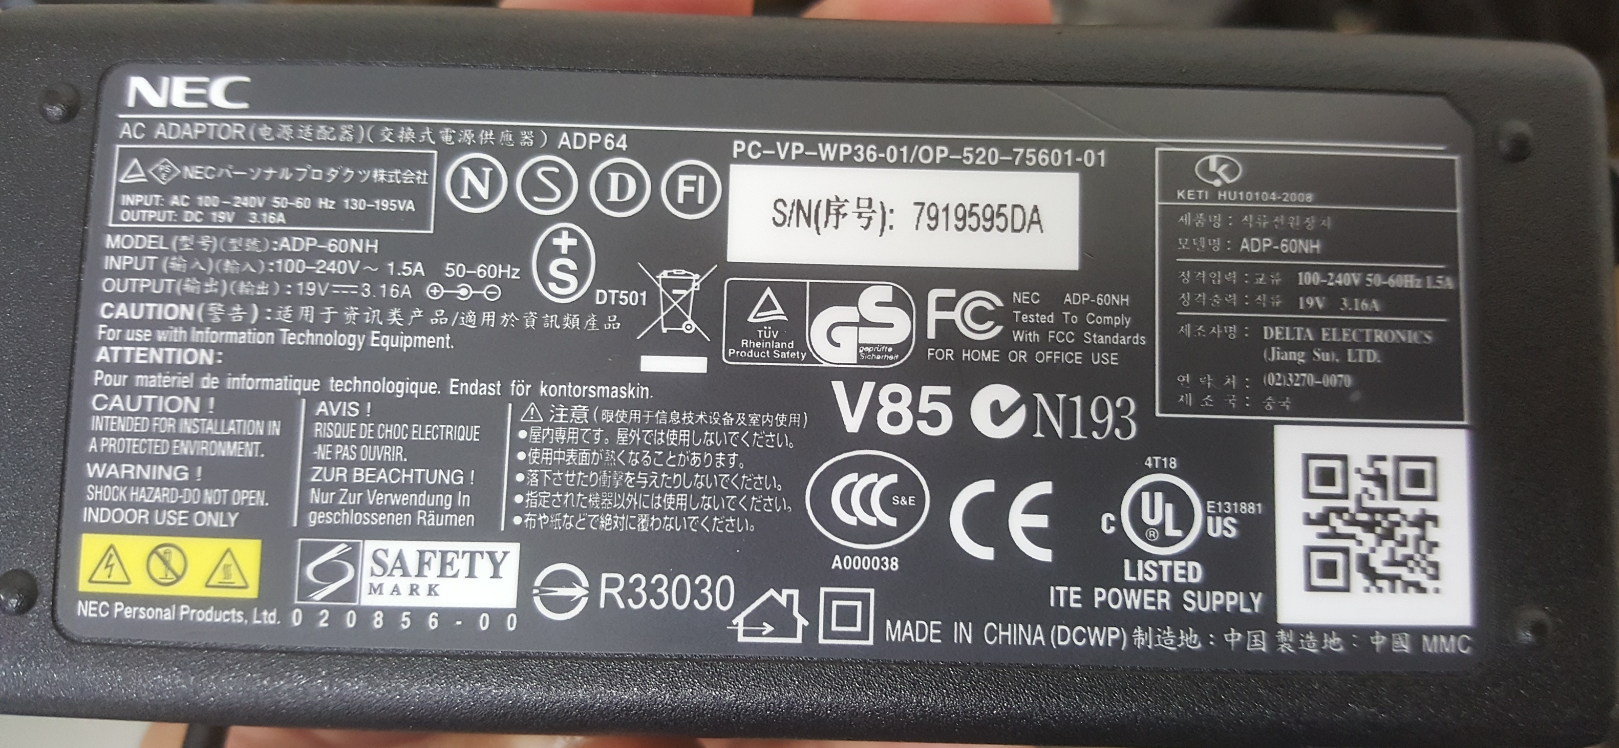
\includegraphics[width=0.48\textwidth]{figure/label-regex-samp.png}
            \end{center}
            \caption{Product label photo.}
            \label{fig:label-regex-samp}
        \end{figure}


%+++++++++++++++++++++++++++++++++++++++++++++++
\section{Proposal of Product Identification System}
\label{sec:proposal}
    In this section, we propose a {\em product identification system} using OCR and a smartphone camera. To identify the product handily, this system obtains the label photo using a smart phone. Then, the product information is extracted by applying OCR to the photo. The {\em fuzzy search} is adopted to improve the accuracy by finding the best-matching record in the database for the possibly incorrect key by OCR. 

    \subsection{System Overview}
        Figure~\ref{fig:system} illustrates the overview of the proposed product identification system. As the system hardware, a {\em smartphone} is used to take a label photo of a target product, to upload the photo to the {\em server}, and to display the identification result to the user. Then, the {\em server} is adopted to run several programs including the web server for the user interface on the smartphone, the interface program to the OCR software, the database system, and the product identification program using {\em FuzzyWuzzy}. 

        \begin{figure}[t] 
            \begin{center}
            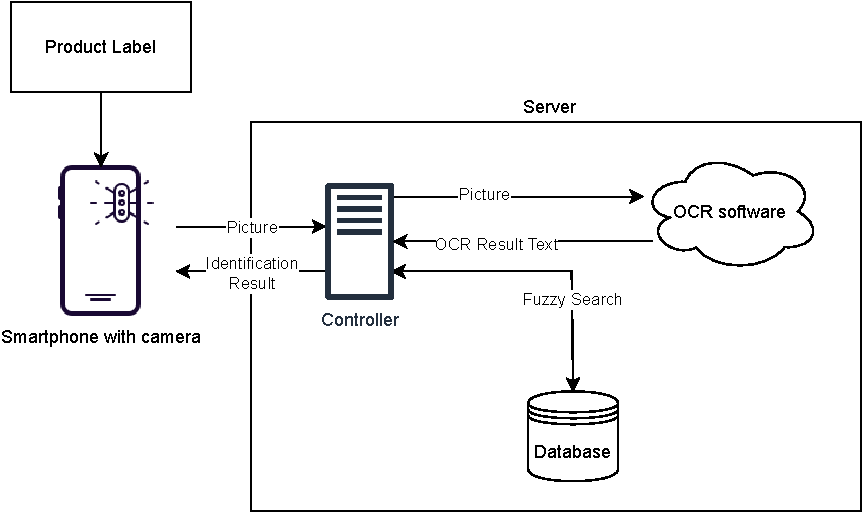
\includegraphics[width=0.48\textwidth]{figure/system.pdf}
            \end{center}
            \caption{System overview.}
            \label{fig:system}
        \end{figure}

    \subsection{System Usage Procedure}
        The usage procedure of the system is described as follows:

        \begin{enumerate}
            \item to take a photo of the product label using a smartphone and upload it to the server using the web browser,
            \item to recognize the characters on the label from the photo using an OCR software on the server,
            \item to extract a set of the candidate strings for the {\em product model number} from the recognized characters by using the {\em regular expression}, 
            \item to calculate the similarity between each candidate string and every records in the database,
            \item to select all the records that have the larger similarity than the given threshold, and display the corresponding product model numbers in descending order of the similarity to the user. 
        \end{enumerate}

        In the following subsections, the details of each step will be explained.

    \subsection{Label Photo by Smarphone}
    \label{sec:label-requirement}
        The user interface for taking the label photo of a product is implemented on a web browser such as Google Chrome with HTML and JavaScript programs. Figure~\ref{fig:homepage} illustrates the web page to take a label photo using a smartphone. By clicking the file selection button on the page, the camera application in the smartphone will be automatically called up.

        \begin{figure}[t] 
            \begin{center}
            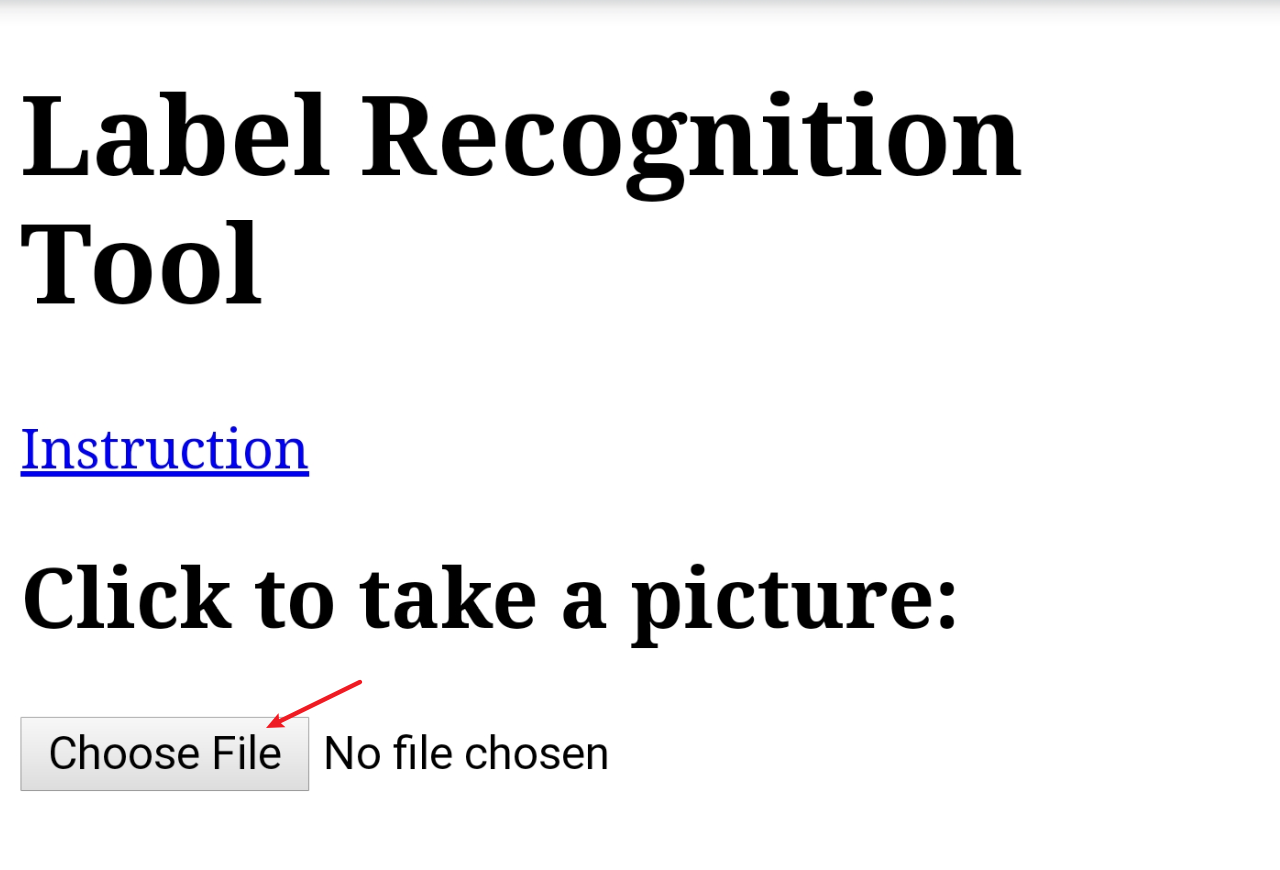
\includegraphics[width=0.35\textwidth]{figure/homepage.png}
            \end{center}
            \caption{Web page for taking photo by smartphone.}
            \label{fig:homepage}
        \end{figure}

        \begin{figure}[t] 
            \begin{center}
            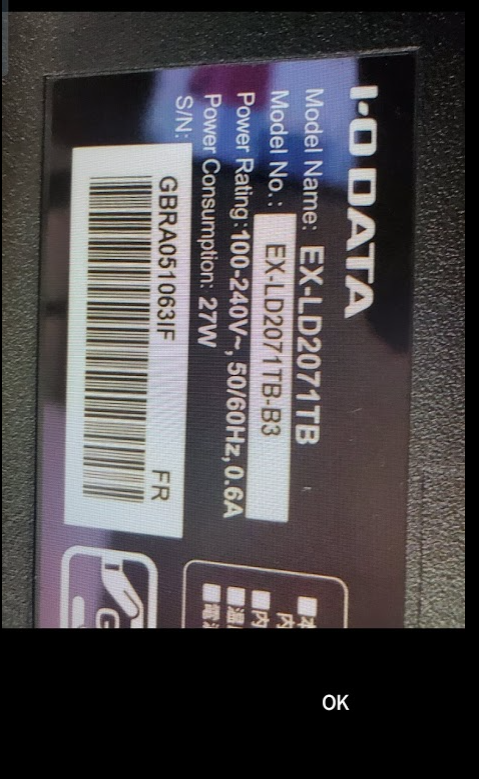
\includegraphics[width=0.30\textwidth]{figure/camera.png}
            \end{center}
            \caption{Smartphone interface after taking photo.}
            \label{fig:camera}
        \end{figure}

        Figure~\ref{fig:camera} shows the user interface on the smartphone after taking a photo. By clicking the “OK” button, the photo will be uploaded to the server. The photo must be taken from the front of the product label. The ambient lighting should be sufficiently good so that the texts on the label can be clearly identified where reflections should be avoided. Besides, the photo should be taken with as few unrelated backgrounds as possible. As the brightness, the contrast, or the other environmental conditions can be changed depending on time and places, the accuracy of the OCR can fluctuate significantly. 

    \subsection{Character Recognition by OCR Software}
        On the server, the label photo is input to an OCR software to recognize the characters in the photo. The accuracy of the system mainly depends on the accuracy of the character recognition results by the OCR software. Unfortunately, we cannot find the commercial OCR software that can avoid a recognition error. Therefore, we propose the following procedure to improve the product identification accuracy of the system by compensating the insufficiency of the OCR software.

    \subsection{Candidate Extraction by Regular Expression}
    \label{sec:regex}
        First, the following {\em regular expression} is applied to the recognized characters by the OCR software, to filter and extract all the alphanumeric strings from them as the candidates to the {\em product model number}:

            \begin{center}
            \begin{BVerbatim}
[ :]*((?=[a-zA-Z0-9\-\/\(\)]*[0-9])
[a-zA-Z0-9\-\/\(\)]{4,})[ ,.]*
            \end{BVerbatim}
            \end{center}
    
        The {\em [ :]*} in the beginning is set to exclude any possible guiding space or colon before the alphanumeric string we need. Then, in the long expression with the brackets, {\em ((?=[a-zA-Z0-9$\backslash$-$\backslash$/$\backslash$($\backslash$)]*[0-9])[a-zA-Z0-9$\backslash$-$\backslash$/$\backslash$($\backslash$)]\{4,\}) }, the {\em (?=[a-zA-Z0-9$\backslash$-$\backslash$/$\backslash$($\backslash$)]*[0-9])} is called for the positive look-ahead in the regular expression. It asserts that the following alphanumeric string should be ending with a number\cite{lookahead}-\cite{regex-tutorial}. This positive look-ahead indicates what the following string should appear. 

        However, it does not actually pick any string, so that the string may contain a number at the middle rather than at the end. Thus, the following {\em [a-zA-Z0-9$\backslash$-$\backslash$/$\backslash$($\backslash$)]\{4,\})} is the one that actually picks a string that has more than four characters as the length, containing letters, numbers, brackets, hyphen, or slashes, without any space. In other words, the alphanumeric string for the candidate of the {\em product model number} must have more than four characters in the length, by containing letters, numbers, brackets, hyphen, or slashes only.

        At the last of the regular expression, {\em [ ,.]*} is used to exclude any possible following space, comma, or dot after the alphanumeric string, and make sure the string ends at the correct position.

In our implementation, we adopt the {\em regex101} tool \cite{regex101} to apply the regular expression to the recognized characters by the OCR software. Sometimes, the same candidates are extracted because the label can show them several times. To reduce the search time, the duplicated candidates are removed after the extractions.


    \subsection{Example Candidate Extraction}

        \begin{figure}[t] 
            \begin{center}
                \begin{BVerbatim}[commandchars=\\\{\}]
NEC
AC ADAPTOR \textcolor{red}{ADP64}
\textcolor{red}{PC-VP-WP36-01/OP-520-75601-01}
\textcolor{red}{ANEC-Y7097Y} N)(S) (D) (FI
D FI
KETI \textcolor{red}{HU10104-2008}
INPUT: AC \textcolor{red}{100-240V 50-60} Hz \textcolor{red}{130-195VA}
OUTPUT: DC 19V 3.16A
S/N(IF ): \textcolor{red}{7919595DA}
MODEL ( O:\textcolor{red}{ADP-60NH}
INPUT (A)(MA):100-\textcolor{red}{240V}~ 1.5A \textcolor{red}{50-60HZ} S
OUTPUT()():19V==3.16A ODO
\textcolor{red}{ADP-60NH}
MARK
NEC Personal Products, Ltd. 0 2 0 85 6 -0 0
                \end{BVerbatim}
            \end{center}
            \caption{Example of candidate extraction results by regular expression.}
            \label{fig:result-regex}
        \end{figure}

        Figure~\ref{fig:result-regex} shows the candidate extraction results by applying the regular expression to the recognized characters by the OCR software for the label photo in Figure~\ref{fig:label-regex-samp}. Here, the candidates are marked by red, where the correct model number {\em ADP-60NH} is included. {\em ADP-60NH} is extracted twice. To reduce the search time, the duplicated candidates are removed.

        
    \subsection{Similarity Calculation}
    \label{sec:algorithm.ocrregex}
        Next, if at least one candidate string for the product model number is extracted in the previous step, the similarity between each candidate string and every corresponding record in the database is calculated using {\em FuzzyWuzzy}. For this purpose, the database should be prepared in advance to contain the related data for any possible product to be identified by the system. Table~\ref{table:db-sample} shows a part of this database. The number of records in this database increases as the number of products to be identified by the system increases. As a result, the CPU time for the similarity calculation by {\em FuzzyWuzzy} can be inhibitory long as the user interactive system.

        \begin{table}[tb]
            \caption{Part of database records.}
            \label{table:db-sample}
            \begin{center}
                \begin{tabular}{l|l}
                    \Hline
                    product\_name & model\_number \\
                    \Hline
                    I-O DATA & EX-LD2071TB \\
                    CM 690 III & CMS-693-KKN1-JP \\
                    EVO Plus & MB-MC128GA \\
                    dynabook PC & PT45NWY-SHA \\
                    ThinkPad X1 Tablet & 20GH-A06VJP \\
                    GALAXY TAB A & SM-T510 \\
                    ThinkSystem & ST50 \\
                    au & T003 \\
                    ideapad S340-14IIL & 81VV \\
                    bizhub & 224e \\
                    COREFIDO & B820n \\
                    ThinkCentre & M900 Small \\
                    dynabook & PT45UWP-SWA \\
                    Smart-UPS 750 & SUA750JB \\
                    dynabook & AZ25/CW \\
                    dynabook Celeron HD & AZ25/B \\
                    dynabook & AZ25/CB \\
                    dynabook Celeron & AZ25/DR \\
                    dynabook Celeron & AZ25/DW  \\
                    HP EliteBook 830 G6 & 8AZ25PA\#ABJ \\
                    PageWide XL & XL 8000 \\                  
                    \Hline
                \end{tabular}
            \end{center}
        \end{table}

    \subsection{System Output}
        Finally, the system outputs all the product model numbers in the database that have the $70$ or higher similarity in descending order. Since the OCR accuracy is not high enough, the system outputs any possible candidate of the product model number, and asks the user to choose one from them manually to improve the accuracy. In most cases, the first candidate is the correct one because it has the highest similarity. Figure~\ref{fig:result-sample} shows the output to the label photo in Figure~\ref{fig:camera}. Here, seven candidates for the product model number are displayed, and the first one is correct.

        \begin{figure}[t] 
            \begin{center}
                \begin{BVerbatim}
Matched Model:
{
    "EX-LD2071TB": 100,
    "EX-LDGC271TB": 87,
    "EX-LD2071TNV": 87,
    "EX-LDQ271DB": 82,
    "EX-LDH271DB": 82,
    "100-MR140": 71,
    "100-LA024": 71
}
                \end{BVerbatim}
            \end{center}
            \caption{Example system output.}
            \label{fig:result-sample}
        \end{figure}


%+++++++++++++++++++++++++++++++++++++++++++++++
\section{Proposal of Speedup Method for Fuzzy Search}
\label{sec:speedup}
    In this section, we present the speedup method for the fuzzy search in the system by limiting the records of product model numbers for the similarity calculation.

    \subsection{Idea of Record Limitation}
        In the naïve logic, the most time-consuming procedure is the {\em similarity calculation} using {\em FuzzyWuzzy}, since the similarity between the candidate strings extracted from the OCR software output and all the records in the database have to be calculated. For the speedup, we limit the number of records in the database for the similarity calculations. Actually, before the similarity calculations, any record that has the same part as the specified part of each candidate string. Then, the similarity is calculated against the selected record only.

    \subsection{Specified String Part}
        In this study, for the specified candidate string part, the first half and the second half of the string are considered. It has been observed that in most cases of the OCR recognition results, the number of incorrectly recognized characters does not exceed one. 
Thus, either of the two half strings have the correct characters of the target product model number with the high probabilities. In our implementation, each extracted candidate string is divided into two halves at the center of the string, and each half string is used in the following partial word matching.

    \subsection{Partial Word Matching}
For each half candidate string, the partial word matching is applied against every record of the product model number in the database. Table~\ref{table:half_matching} shows one example of this procedure. Here, the correct product model number is “AZ25/CB”, but the extracted candidate string by the regular expression from the OCR software output is “AZ25/C8”, which has one error of “8” instead of “B”. Then, this candidate string is divided into two halves, “AZ25” and “/C8”. 

After that, each half string is used in the partial word matching with every record in the database. Then, “AZ25” finds the four records including the correct one, and “/C8” does no record. The similarity calculations are applied against only these four records, which can drastically reduce the number of matching records and speed up the similarity calculations.

        \begin{table}[tb]
            \caption{Example of record limitation.}
            \label{table:half_matching}
            \begin{center}
                \begin{tabular}{c|c|c}
                \Hline
                product model number & \multicolumn{2}{c}{AZ25/CB} \\ 
                \hline
                extracted candidate string & \multicolumn{2}{c}{AZ25/C{\em 8}} \\ 
                \hline
                half strings & \_\_AZ25\_\_ & \_\_/C{\em 8}\_\_ \\
                \hline
                matching records & \begin{tabular}{c}AZ25\underline{/CB}\\AZ25\underline{/B}\\AZ25\underline{/CW}\\\underline{8}AZ25\underline{PA\#ABJ}
\end{tabular} & (no result) \\
                \Hline
                \end{tabular}
            \end{center}
        \end{table}
        
%+++++++++++++++++++++++++++++++++++++++++++++++
\section{Evaluation}
\label{sec:evaluation}
    In this section, we evaluate the proposal in this study. For evaluations, we collect 396 label photos of different products using the system.

    \subsection{Evaluation of Candidate String Extraction}
    \label{sec:regex-result}
First, we evaluate the candidate string extraction accuracy by our proposal. 
Table~\ref{table:regex_result} shows the summary of candidate string extraction results for the $396$ product label photos by the proposal. In this table, the {\em fully correct number} indicates the results for the label photos such that the output of the proposal includes the fully correct product model number that has no error. The {\em partially correct number} indicates the results such that the output includes the partially correct number that has some different characters from the correct one. The {\em no correct number} indicates the results such that the output does not include even the partially correct number.

        \begin{table*}[t]
            \caption{Candidate string extraction results.}
            \label{table:regex_result}
            \begin{center}
                \begin{tabular}{c|cccc}
                \Hline
                    item & \begin{tabular}{c}fully correct\\ number\end{tabular} & \begin{tabular}{c}partially correct\\ number \end{tabular} & \begin{tabular}{c}no correct\\ number \end{tabular} & total \\ 
                \hline
                number of photos & 311 & 78 & 7 & 396 \\
                percentage (\%) & 78.5 & 19.7 & 1.8 & 100.0 \\
                Average number of extracted candidates & 8.39 & 10.13 & 3.86 & 8.65 \\ 
                % \hline
                Maximum number of extracted candidates & 38 & 23 & 8 & 38 \\ 
                % \hline
                Minimum number of extracted candidates & 1 & 1 & 2 & 1 \\ 
                \Hline
                \end{tabular}
            \end{center}
        \end{table*}

       Table~\ref{table:regex_result} suggests that the OCR software and the regular expression in the proposal can extract the fully correct records for the $311$ photos or $78.5\%$ among the $396$ photos, and the partially correct records for the $78$ photos or $19.7\%$. For them, the fuzzy search using the similarity calculations can detect the correct records in the database.

However, it cannot extract even the partially correct records for the $7$ photos or $1.8\%$. In these photos, most of the product model numbers are very short. The improvements of the proposal for such numbers will be in future works.
        
The average number of extracted candidates from one photo is $8.65$. As this number increases, the record search time using the fuzzy search increases. Thus, the reduction of this number will also be in future works.


    \subsection{Evaluation of Number Recognition}
           
For the extracted candidates for the $389$ photos at {\em fully correct number} or at {\em partially correct number} in Table~\ref{table:regex_result}, the fuzzy search is conducted to the $553,887$ records in the database for the system. Here, both the naïve method and the speedup method are applied. Table~\ref{table:methods_compare} shows the summary of the product model number recognition results to the $396$ photos by the proposal. In this table,                {\em correct number with max. score} indicates the number of photos such that the model number in the output has the largest score. {\em correct number with other score} indicates the number of photos such that the model number in the output has the other score to the largest. {\em number of failed photos} indicates the number of photos such the model number does not appear in the output. 

        \begin{table*}[t]
            \caption{Application results.}
            \label{table:methods_compare}
            \begin{center}
                \begin{tabular}{l|ccc|ccc}
                \Hline
                search method &
                    \multicolumn{3}{c|}{naïve method} &
                    \multicolumn{3}{c}{speedup method} \\ 
                \hline
                Regular expression result &
                    fully & partially & total & 
                    fully & partially & total & 
                \hline
                number of photos &
                    311 & 78 & 389 &
                    311 & 78 & 389 \\
                maximum similarity score &
                    100 & 100 & 100 &
                    100 & 100 & 100 \\ 
                correct number with max. score &
                    307 & 33 & 340 &
                    307 & 32 & 339 \\ 
                correct number with other score &
                    4 & 23 & 27 &
                    4 & 23 & 27 \\ 
                number of failed photos &
                    0 & 22 & 22 &
                    0 & 23 & 23 \\ 
                recognition rate (\%) &
                    100.0 & 71.8 & 94.3 &
                    100.0 & 70.5 & 94.1 \\ 
                average number of outputs &
                    14.56 & 14.79 & 14.60 &
                    12.64 & 12.58 & 12.63 \\ 
                average search time (sec) &
                    14.82 & 17.68 & 15.39 &
                    0.98 & 1.03 & 0.99 \\ 
                minimum search time (sec) &
                    2.04 & 2.07 & 2.04 &
                    0.54 & 0.51 & 0.51 \\ 
                maximum search time (sec) &
                    64.27 & 39.54 & 64.27 &
                    3.00 & 2.51 & 3.00 \\ 
                average number of cal. records &
                    553,887.00 & 553,887.00 & 553,887.00 &
                    1,208.27 & 1,916.88 & 1,350.36 \\
                \Hline
                \end{tabular}
            \end{center}
        \end{table*}

    \subsubsection{Naïve Method}
The naïve method detects the correct number or database record for the $340$ photos with the highest score, where users do not need to choose the correct one from the multiple candidate numbers in the output. The rate for detecting the correct number among all the photos is $94.3\%$. For one photo, the average number of candidate numbers in the output is $14.6$. The average search time is $15.39sec$, and the maximum time is $64.27sec$, where the similarity is calculated against all of the $553,887$ records in the database.
        
    \subsubsection{Speedup Method}
The speedup method detects the correct number or database record for the $339$ photos with the highest score. The rate for detecting the correct number is $94.1\%$. For one photo, the average number of candidate numbers in the output is $12.63$. The average search time is $0.99sec$, and the maximum time is $3sec$, where the similarity is calculated against only the $1350.36$ records or $0.24\%$ of all the records in the database.
The speedup method can effectively reduce the search time into the acceptable range while keeping the accuracy. 

     \subsubsection{Slow Photos}
Table~\ref{table:slowest_rec} shows the slow search results for six photos where even the speedup method takes rather long time. The reason is that the number of extracted candidate strings by the regular expression is large compared with the others. The reduction of them will be in future works for further speedup of the system.        
        
        \begin{table*}[t]
            \caption{Slow search results using speed-up method}
            \label{table:slowest_rec}
            \begin{center}
                \begin{tabular}{c|c|c|c|c|c|c}
                \Hline
                    \begin{tabular}{c}product\\model\\number\end{tabular} &
                    \begin{tabular}{c}number of\\extracted\\candidates\end{tabular} &
                    \begin{tabular}{c}search\\time (s)\end{tabular} &
                    \begin{tabular}{c}number of\\search\\records\end{tabular} &
                    \begin{tabular}{c}maximum\\score\\output\end{tabular} &
                    \begin{tabular}{c}any\\score\\output\end{tabular} &
                    \begin{tabular}{c}maximum\\similarity\\score\end{tabular} \\ 
                \Hline
                DC35 & 14 & 1.80353 & 24,675 & incorrect & incorrect & 89 \\ 
                \hline
                DM-E25AW & 29 & 2.41260 & 2,912 & correct & correct & 100 \\ 
                \hline
                TPC-F026-SF & 23 & 2.51139 & 6,761 & correct & correct & 91 \\ 
                \hline
                K04A-WH & 38 & 2.53164 & 5,009 & correct & correct & 100 \\ 
                \hline
                MRO-GS8 & 22 & 2.91033 & 3,822 & correct & correct & 100 \\ 
                \hline
                NE-BS805-K & 33 & 3.00420 & 5574 & correct & correct & 100 \\ 
                \Hline
                \end{tabular}
            \end{center}
        \end{table*}
      
               
%+++++++++++++++++++++++++++++++++++++++++++++++
\section{Conclusion}
\label{sec:conclusion}
%summary
    In this study, we proposed the {\em product identification system} using the {\em optical character recognition (OCR)} software to the label photo taken by a smart phone. The {\em fuzzy search} is adopted with the speedup method to improve the accuracy by finding the best-matching record of the product model number in the database. The application results to $396$ product label photos showed the effectiveness of the proposal. 
%future works
In future works, we will study to improve the accuracy of the system particularly for labels that have short product model numbers, reduce the number of extracted candidate strings by the regular expression to further reduce the search time. We will also improve the user interface and further investigate the performance of the proposal with various product label photos.

%+++++++++++++++++++++++++++++++++++++++++++++++
%\bibliographystyle{sieicej}
%\bibliography{myrefs}
\begin{thebibliography}{99}% 文献数が10未満の時 {9}
    \bibitem{fuzzywuzzy-guidence}
    “FuzzyWuzzy: Fuzzy string matching in Python, beginner’s guide,” Towards Data Science, 
\url{https://towardsdatascience.com/fuzzywuzzy-fuzzy-string-matching-in-python-beginners-guide-9adc0edf4b35}.

    \bibitem{string-correction}
    R. A. Wagner and M. J. Fischer, “The string-to-string correction problem,“ J. ACM, vol. 21, no. 1, pp. 168-173, 1974.

    \bibitem{guide-to-matching}
    G. Navarro, “A guided tour to approximate string matching, ACM Comput. Surv., vol. 33, no. 1, pp. 31–88, 2001.

    \bibitem{levenshtein}
    “Levenshtein distance,” Wikipedia,
 \url{https://en.wikipedia.org/wiki/Levenshtein_distance}.

    \bibitem{fuzzywuzzy}
“FuzzyWuzzy: Fuzzy string matching in Python,” ChairNerd, July 2011, \url{https://chairnerd.seatgeek.com/fuzzywuzzy-fuzzy-string-matching-in-python/}.

    \bibitem{fuzzywuzzy-git}
    “FuzzyWuzzy,” GitHub, \url{https://github.com/seatgeek/fuzzywuzzy}.

    \bibitem{lookahead}
    J. Goyvaerts, “Positive and negative Lookahead,” Regular-Expressions.info., 2020, \emph{\url{https://www.regular-expressions.info/lookaround.html}

    \bibitem{lookahead-and-behind}
    “Regular expressions - lookahead and lookbehind,” SO Documentation, \url{https://sodocumentation.net/regex/topic/639/lookahead-and-lookbehind}.

    \bibitem{regex-tutorial}
    RegexTutorial, “Regex Lookahead,” \url{https://www.regextutorial.org/positive-and-negative-lookahead-assertions.php}.

    \bibitem{regex101}
  regular expressions 101, Regex101, \url{https://regex101.com/}.

\end{thebibliography}

\end{document}


